\documentclass{article}
\usepackage[utf8]{inputenc}
\usepackage[english]{babel}
\usepackage{graphicx}

\usepackage{hyperref}

\usepackage{xcolor}

\title{Report}
\author{Egirin Gega \&  Samuli Romo}

\begin{document}
  \maketitle

  \newpage
  \tableofcontents
  \newpage
  \listoffigures

  \newpage
  \section{Convolutional Neural Network}
  A Convolutional Neural Network also known as a CNN or COMV NET is an artificial neural network that is so far been most popularly used for analyzing images. Although image analysis has been the most widespread use of CNN's they can also be used for other data analysis or classification problems as well most generally.
  \subsection{How does it Work}
    \subsubsection{Filters}
    The idea behind a convolutional neural network is that you filter the images before training the deep neural network. After filtering the images, features within the images could then come to the forefront and you would then spot those features to identify something.
    A filter is simply a set of multipliers. 
    \vspace{20mm}
    \begin{figure}[h!]
      \begin{center}
        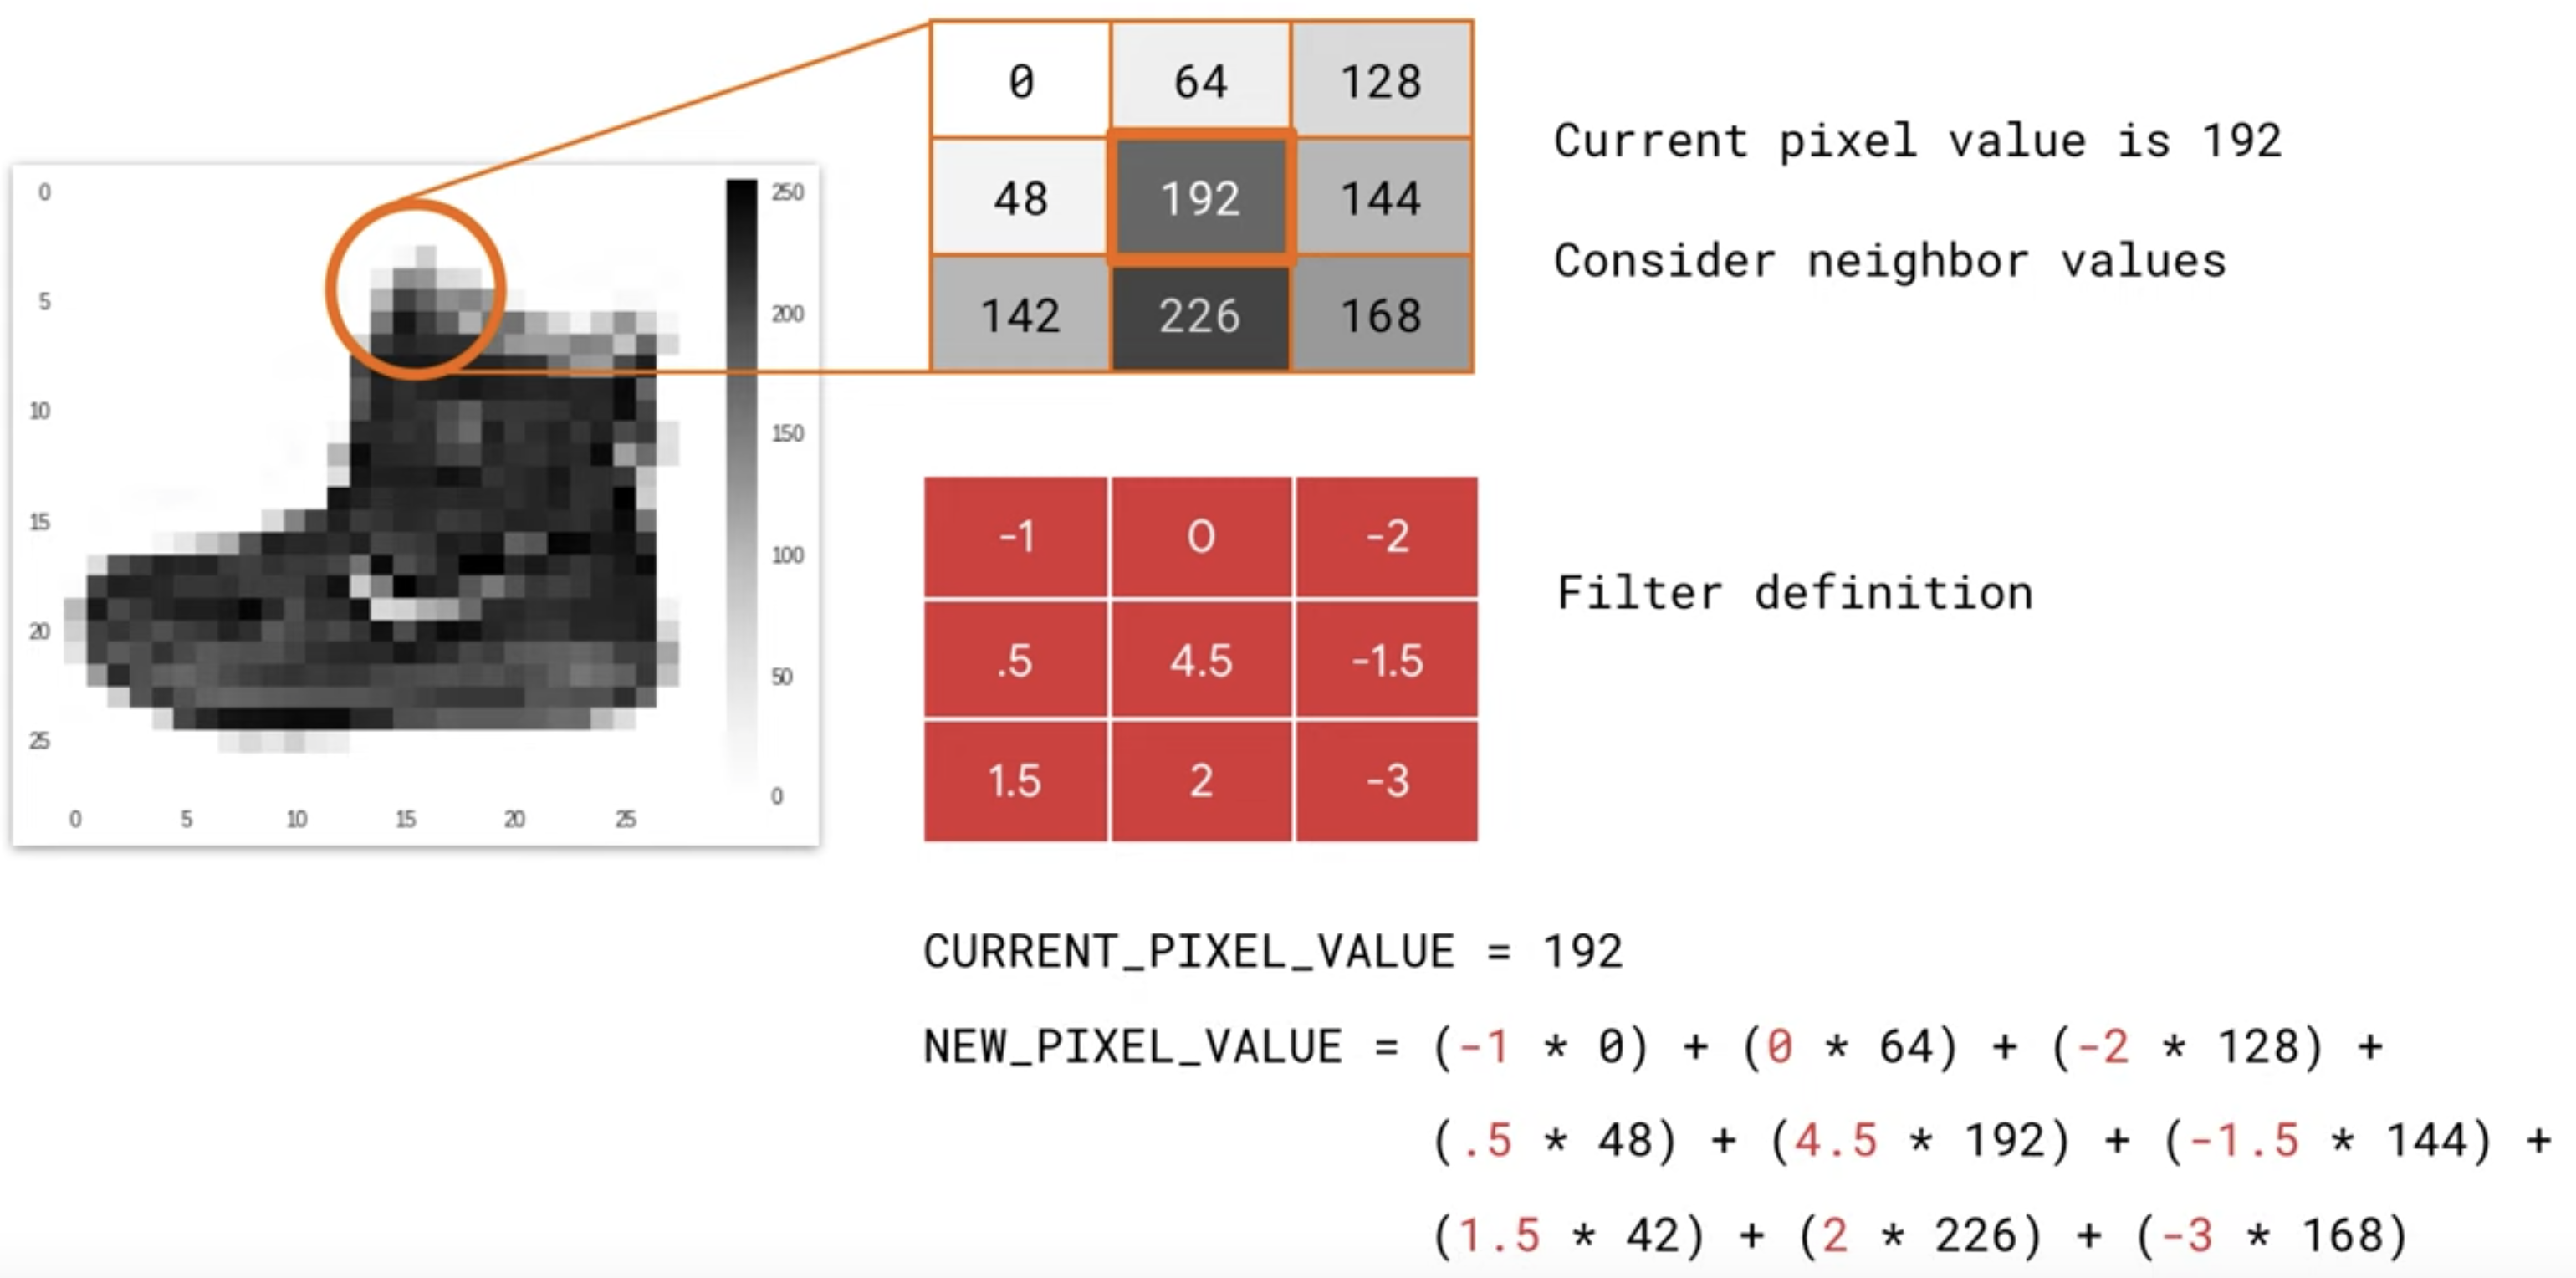
\includegraphics[width=\linewidth]{img/img2.png}
        \caption{Object image}
        \label{fig:snn}
      \end{center}
    \end{figure}
    \paragraph{}
    So, for example, in this case, if you're looking at a particular pixel that has the value 192 and the filter is the values in the red box then you multiply 192 by 4.5, and each of its neighbors by the respective filter value. So it`s neighbor above and to the left is 0, so you multiply that by -1. Its upper neighbor is 64 so you multiply that by 0 and so on. Sum up the result and you get the new value for the pixel.
    \begin{figure}
      \centering
      \begin{minipage}{.5\textwidth}
        \centering
        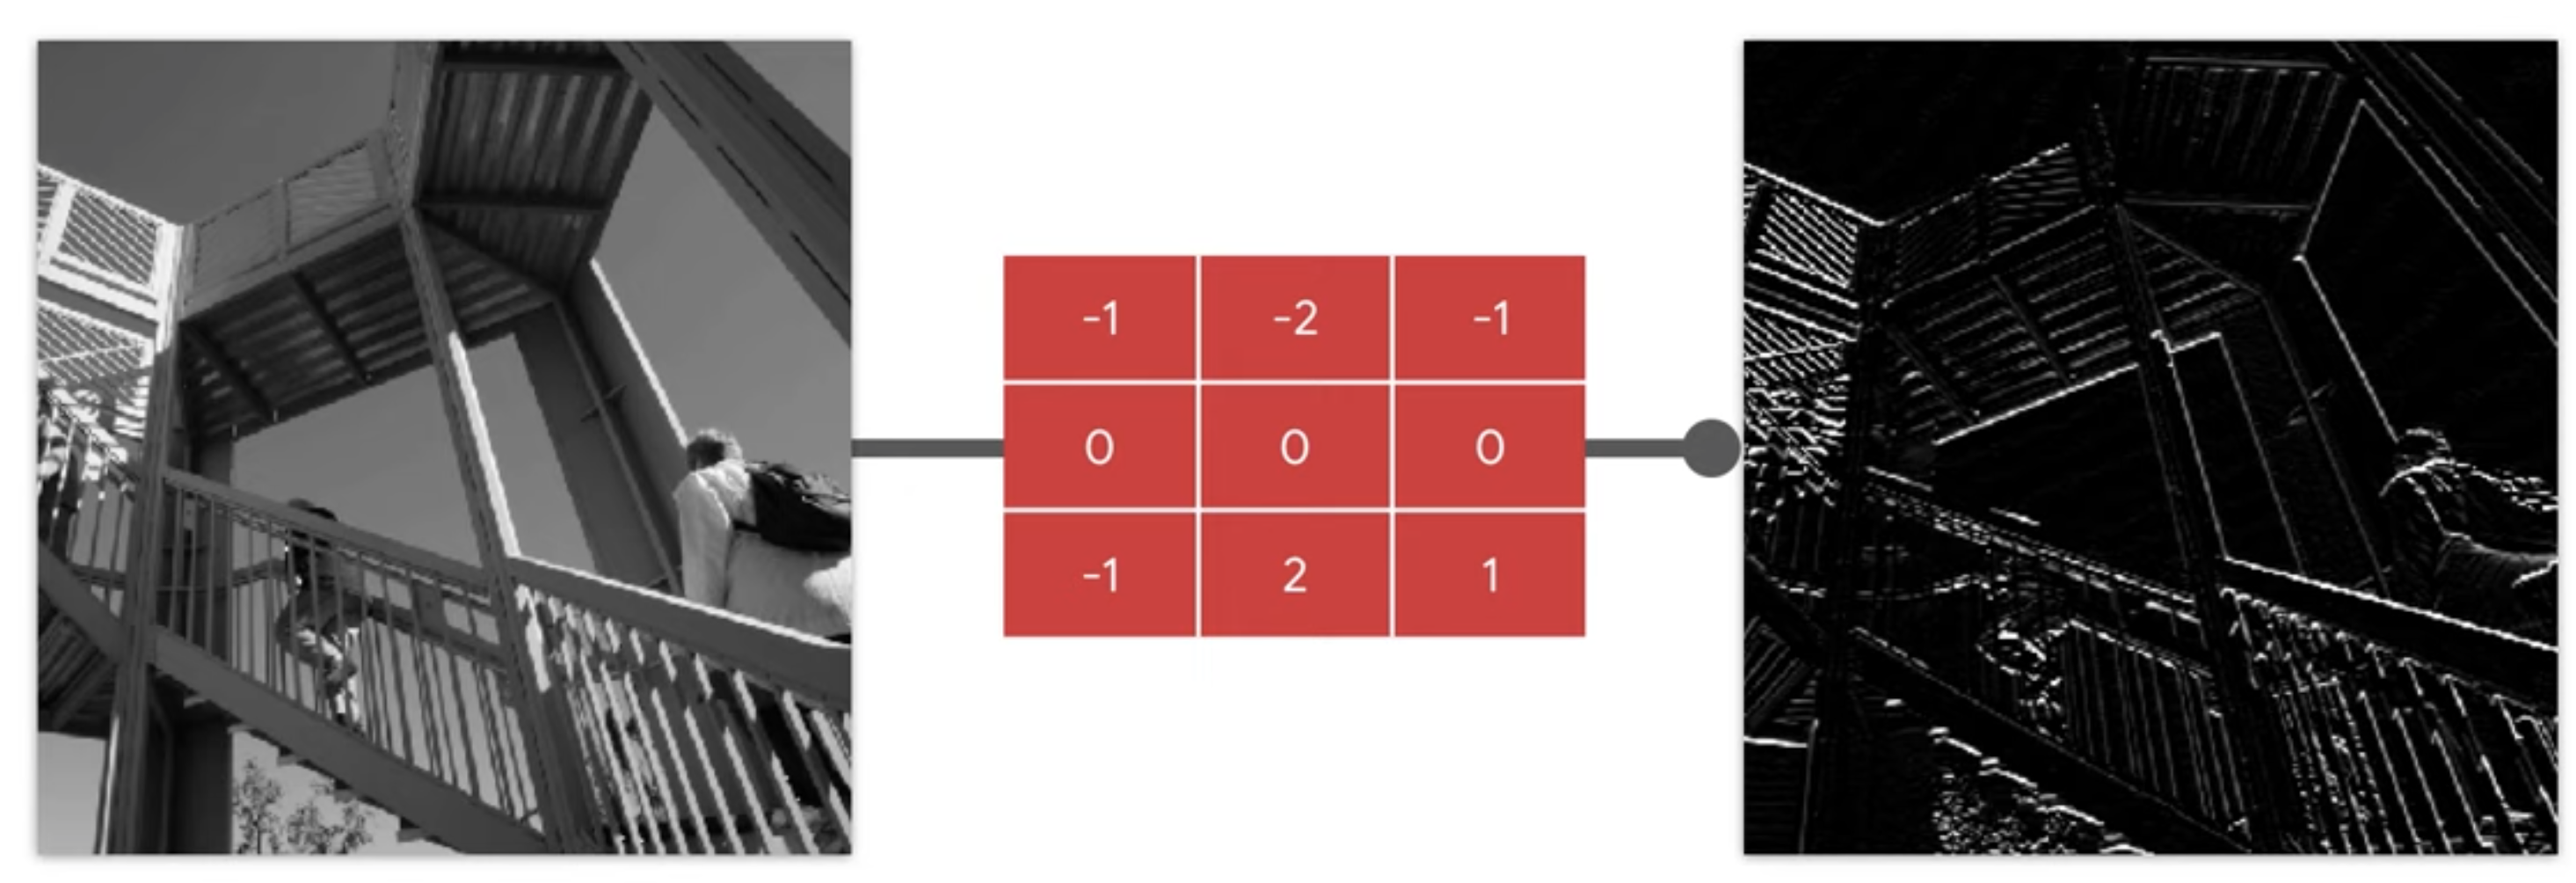
\includegraphics[width=0.9\linewidth]{img/h-line.png}
        \caption{Horzontal line filter}
        \label{fig:test1}
      \end{minipage}%
      \begin{minipage}{.5\textwidth}
        \centering
        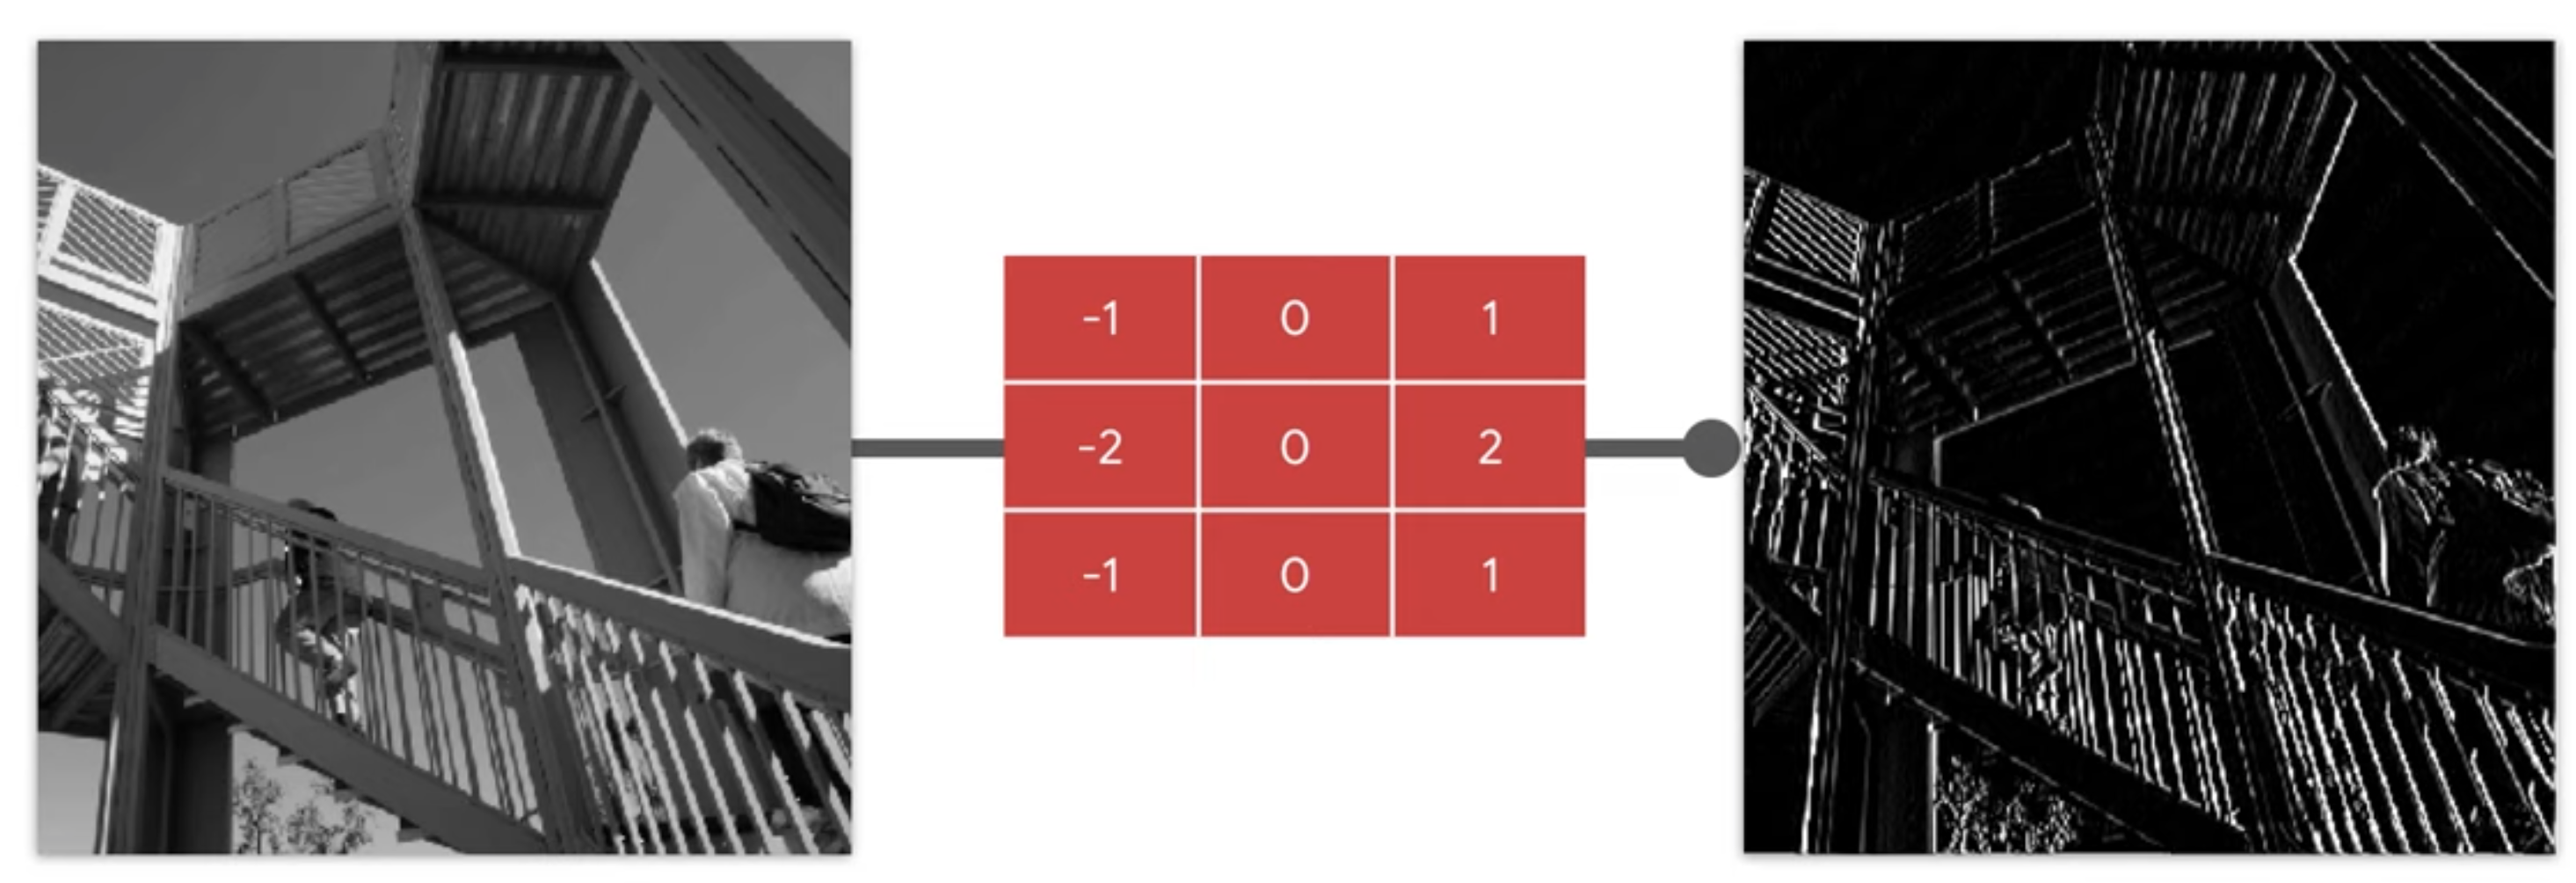
\includegraphics[width=0.9\linewidth]{img/v-line.png}
        \caption{Vertical line filter}
        \label{fig:test2}
      \end{minipage}
    \end{figure}
    \paragraph{}
    Now this might seem a little odd but checkout the results for some filters like this one, that when multiplied over the contents of the image, it removes almost everything except the vertical lines. And this one that removes almost everything except the horizontal lines.
    \vspace{10mm}
    \begin{figure}[h!]
      \begin{center}
        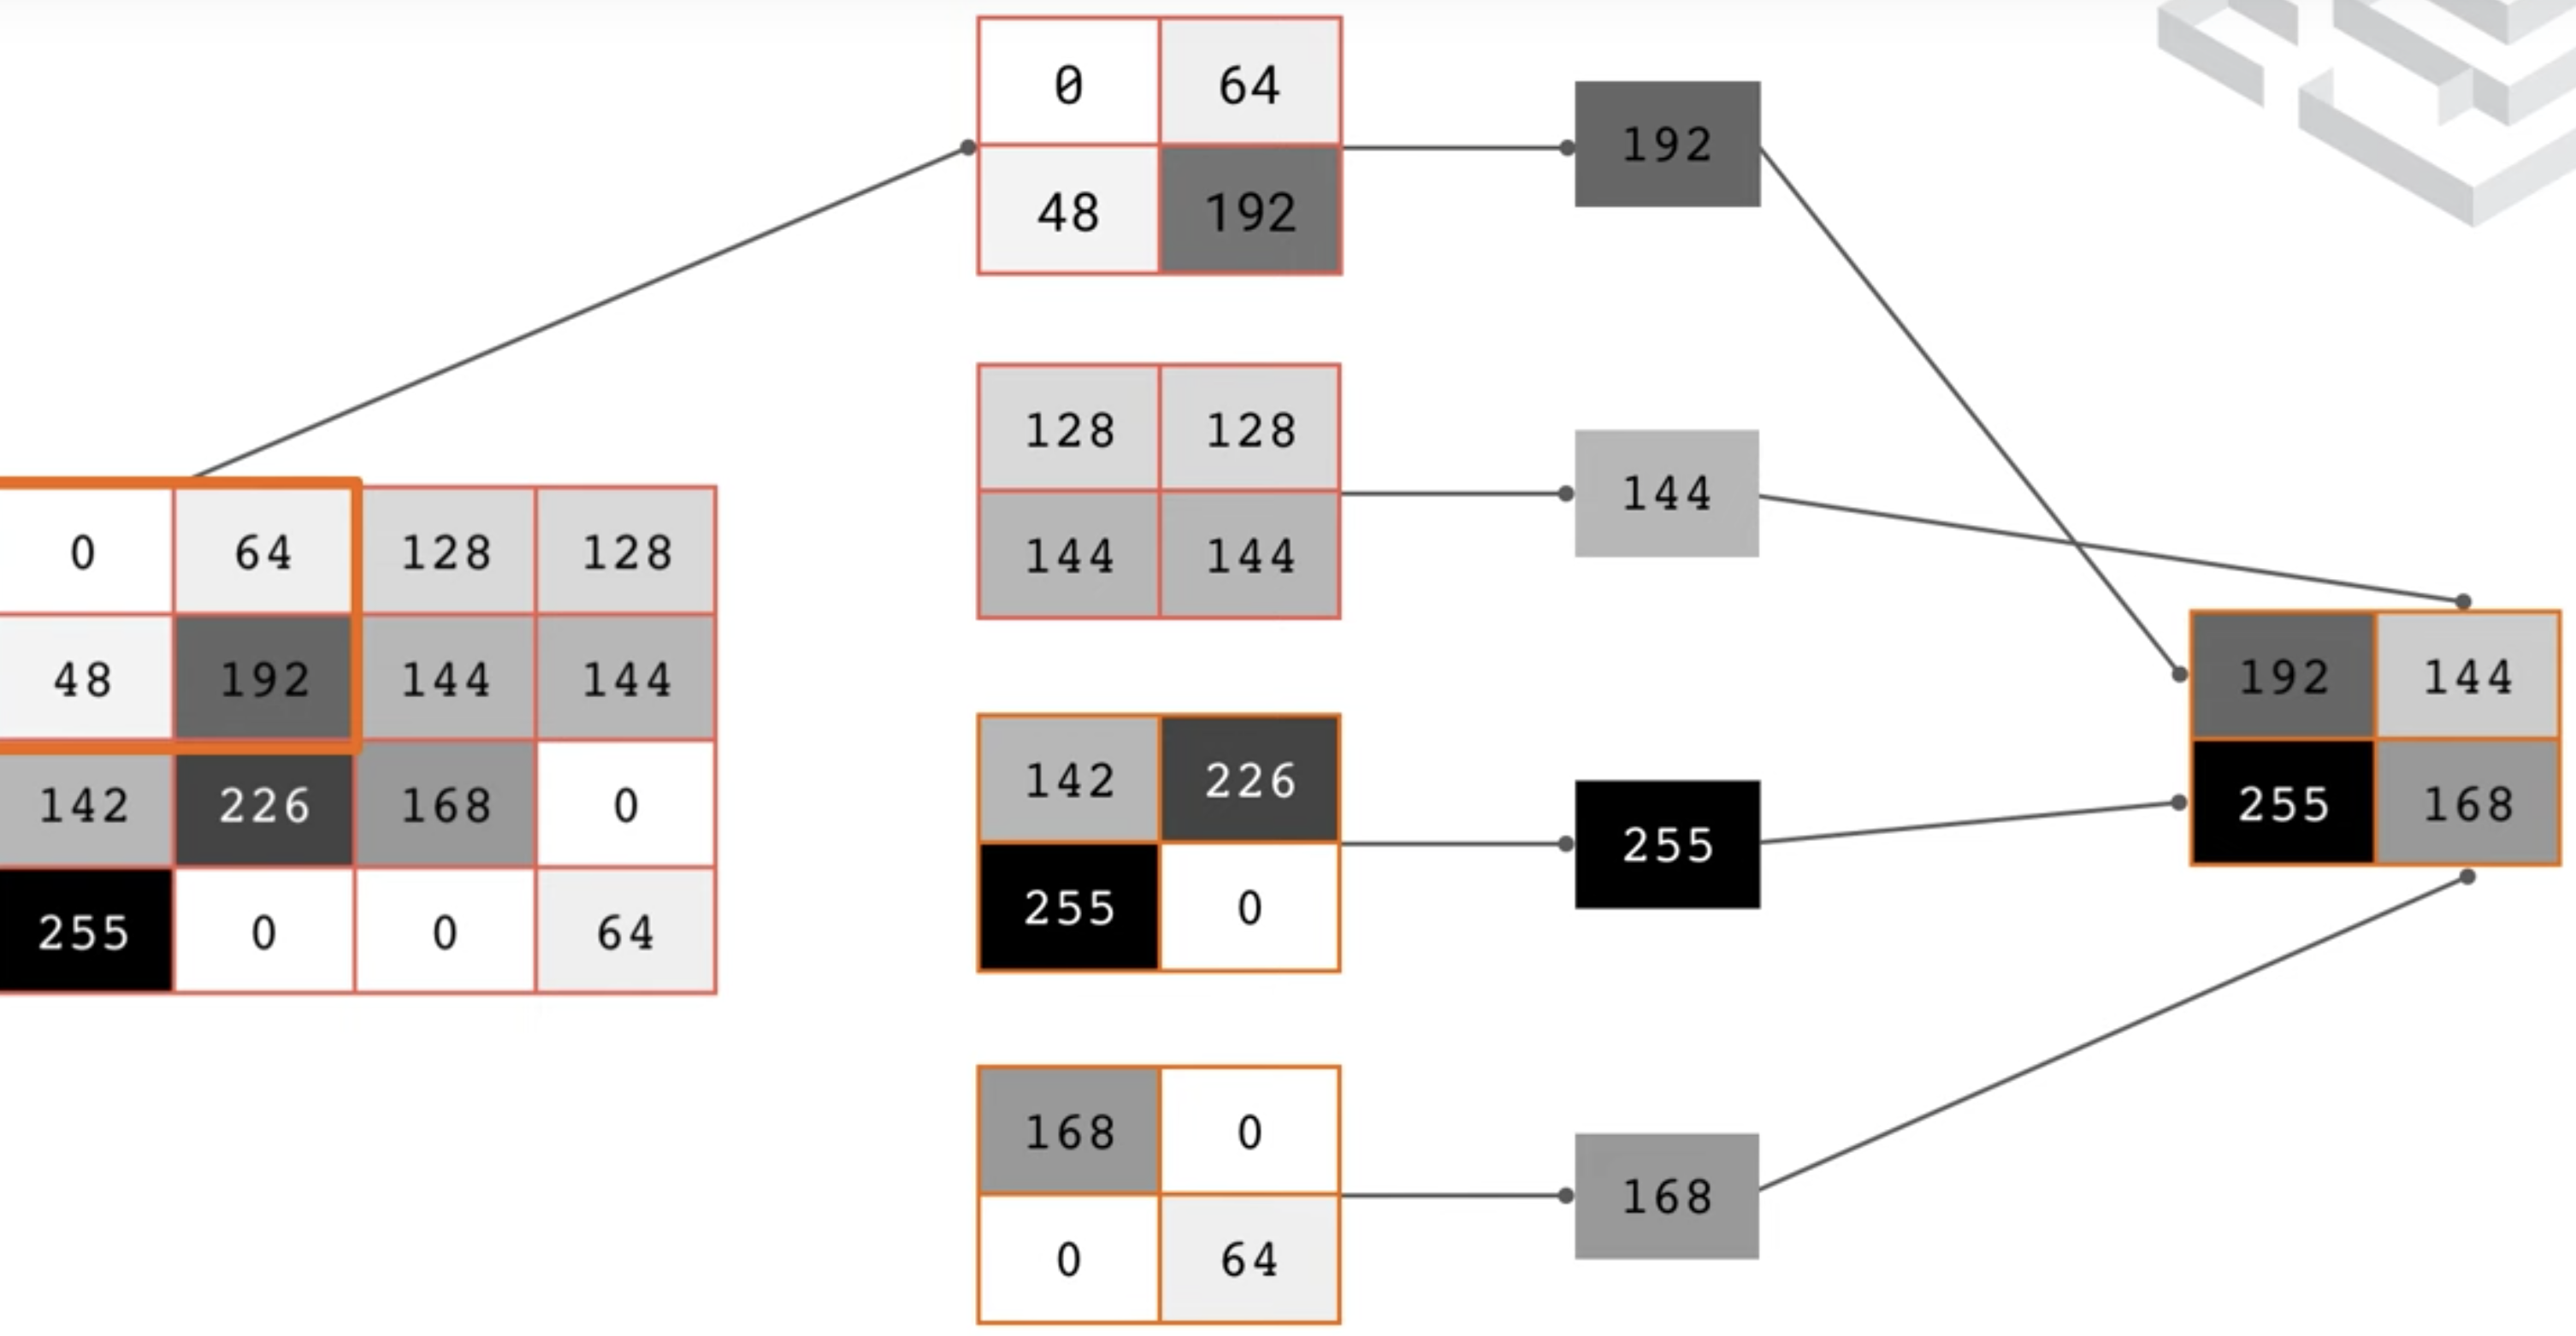
\includegraphics[width=0.7\linewidth]{img/comp.png}
        \caption{Combination Max Pooling}
        \label{fig:snn}
      \end{center}
    \end{figure}
    \subsubsection{Max Pooling}
    This can then be combined with something called pooling, witch. groups up pixels in the image and filters them down to a subset. So for example max pooling 2x2 will group the image into sets of 2x2 pixels and simply pick the largest. the image will be reduced into a quarter of its original size but the features can still be maintained. 
    \vspace{40mm}
    \begin{figure}[h!]
      \begin{center}
        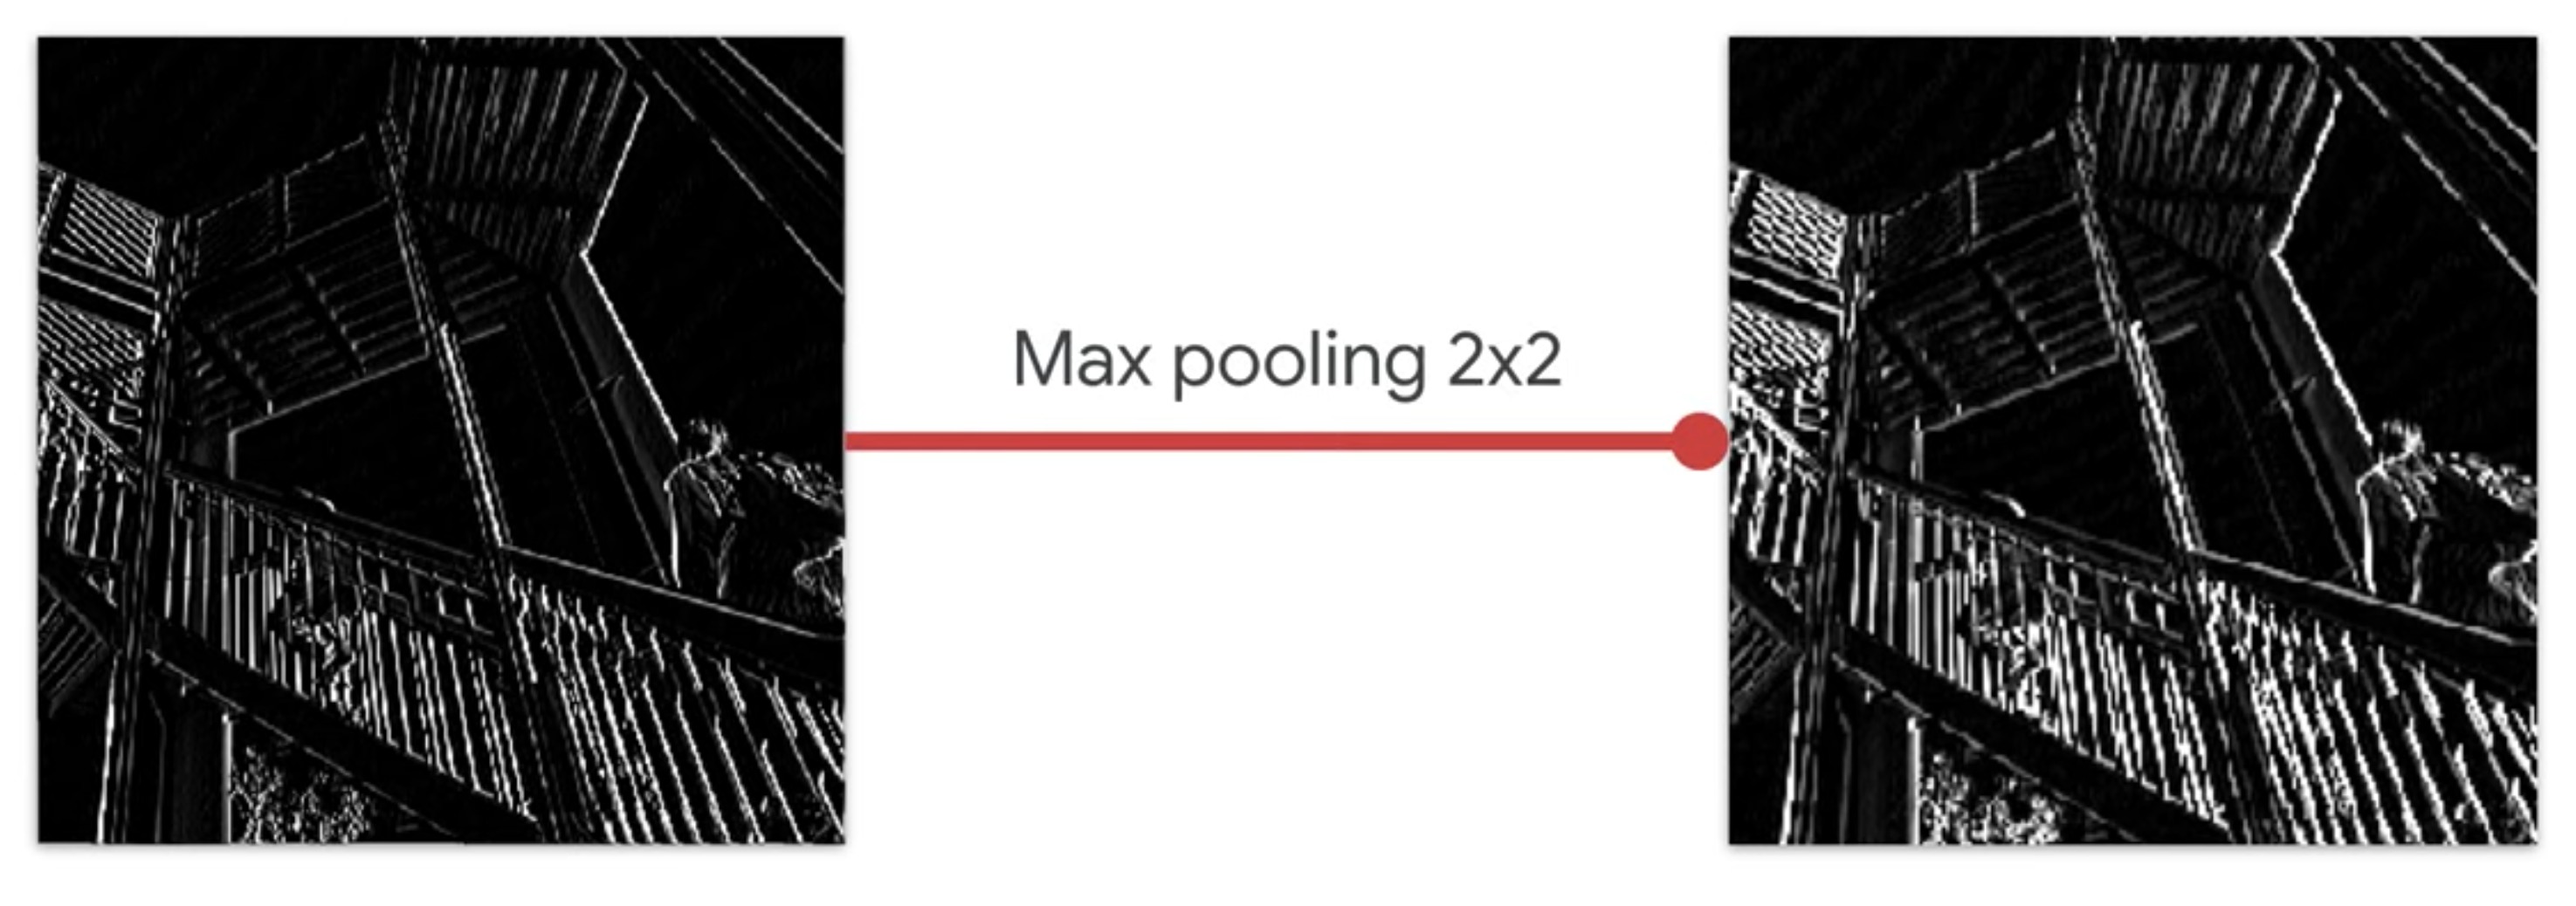
\includegraphics[width=0.7\linewidth]{img/maxpool.png}
        \caption{Max Pooling}
        \label{fig:snn}
      \end{center}
    \end{figure}
    \paragraph{}
    So the previous image after being filtered and then max pooled could look like this. The image on the right is one quarter of the one on the left, but the vertical line features where maintained and indeed they where enhanced.

    \vspace{10mm}
    \begin{figure}[h!]
      \begin{center}
        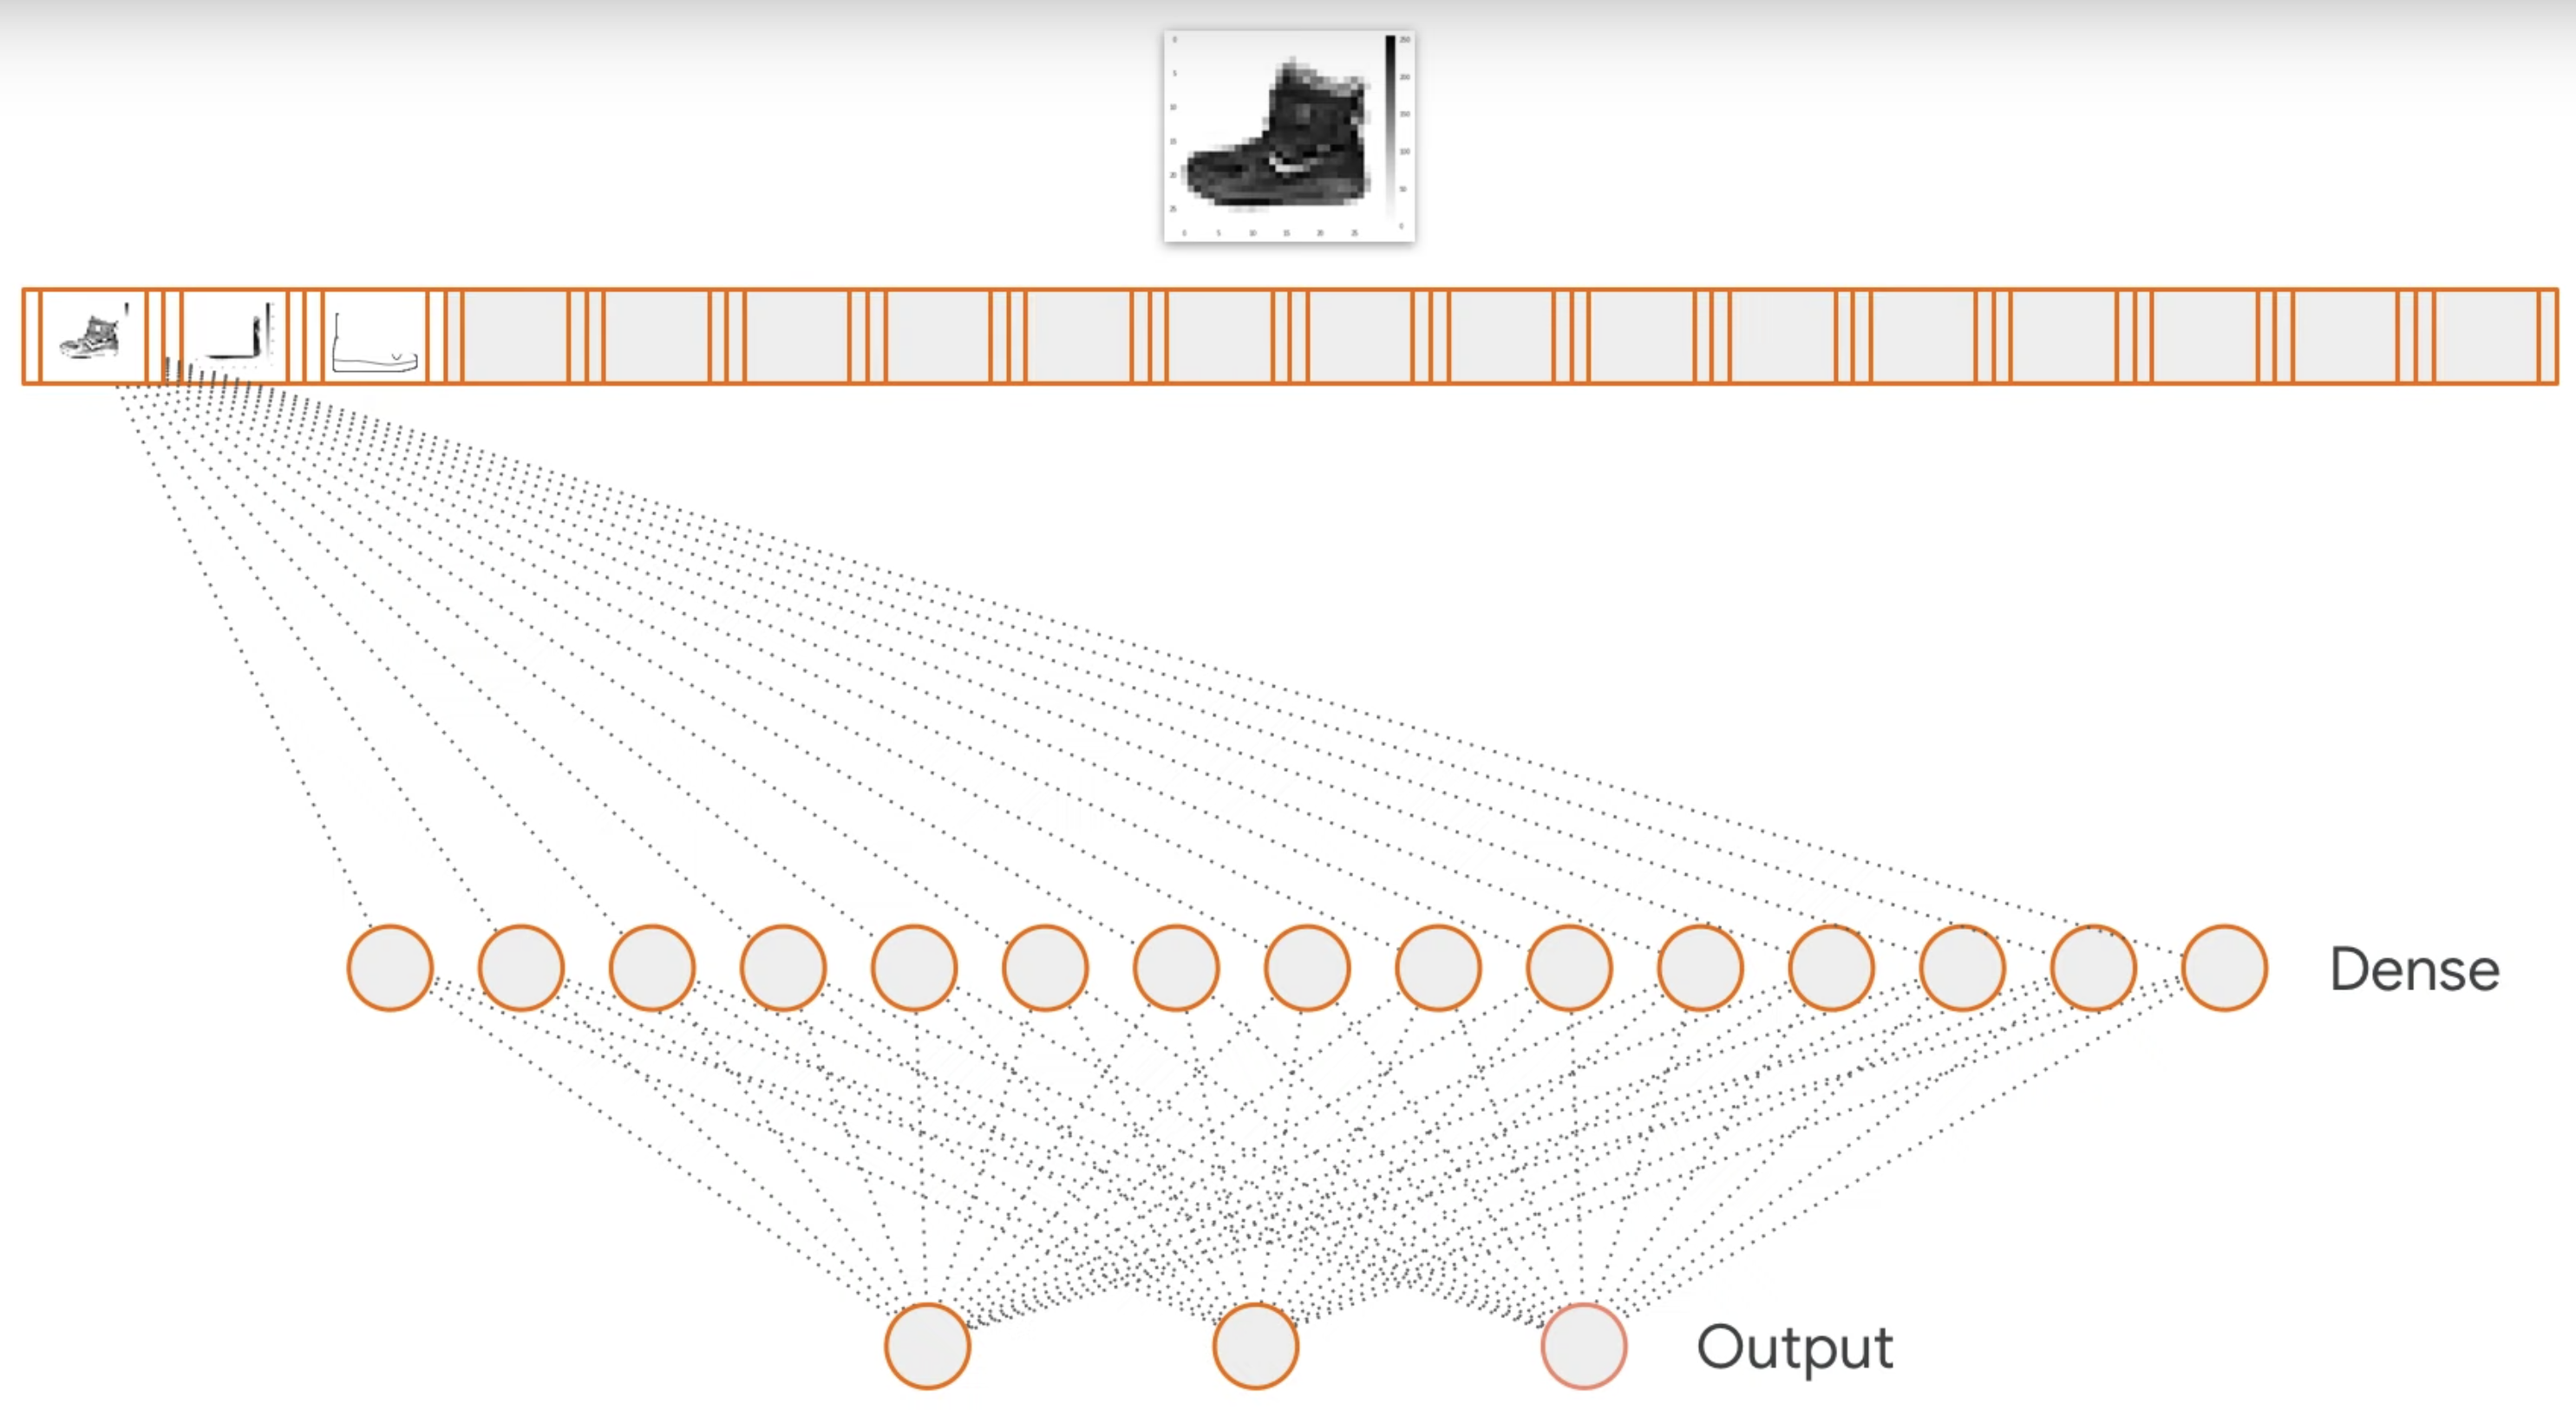
\includegraphics[width=0.7\linewidth]{img/features.png}
        \caption{Features}
        \label{fig:snn}
      \end{center}
    \end{figure}
    \subsubsection{Code sample}
    So where did these filters come from? Thats the magic of a convolutional neural network. They`re actually learned. They are just parameters like those on the neurons of a neural network. So as our image is feed into the convolutional layer, a number of randomly initialized filters will pass over the image. The results of these are fed into the next layer and matching is performed by the neural network. And overtime the filters that gave us the image outputs that give the best matches will be learned and the process is called feature extraction. 
    \vspace{10mm}
    \begin{figure}[h!]
      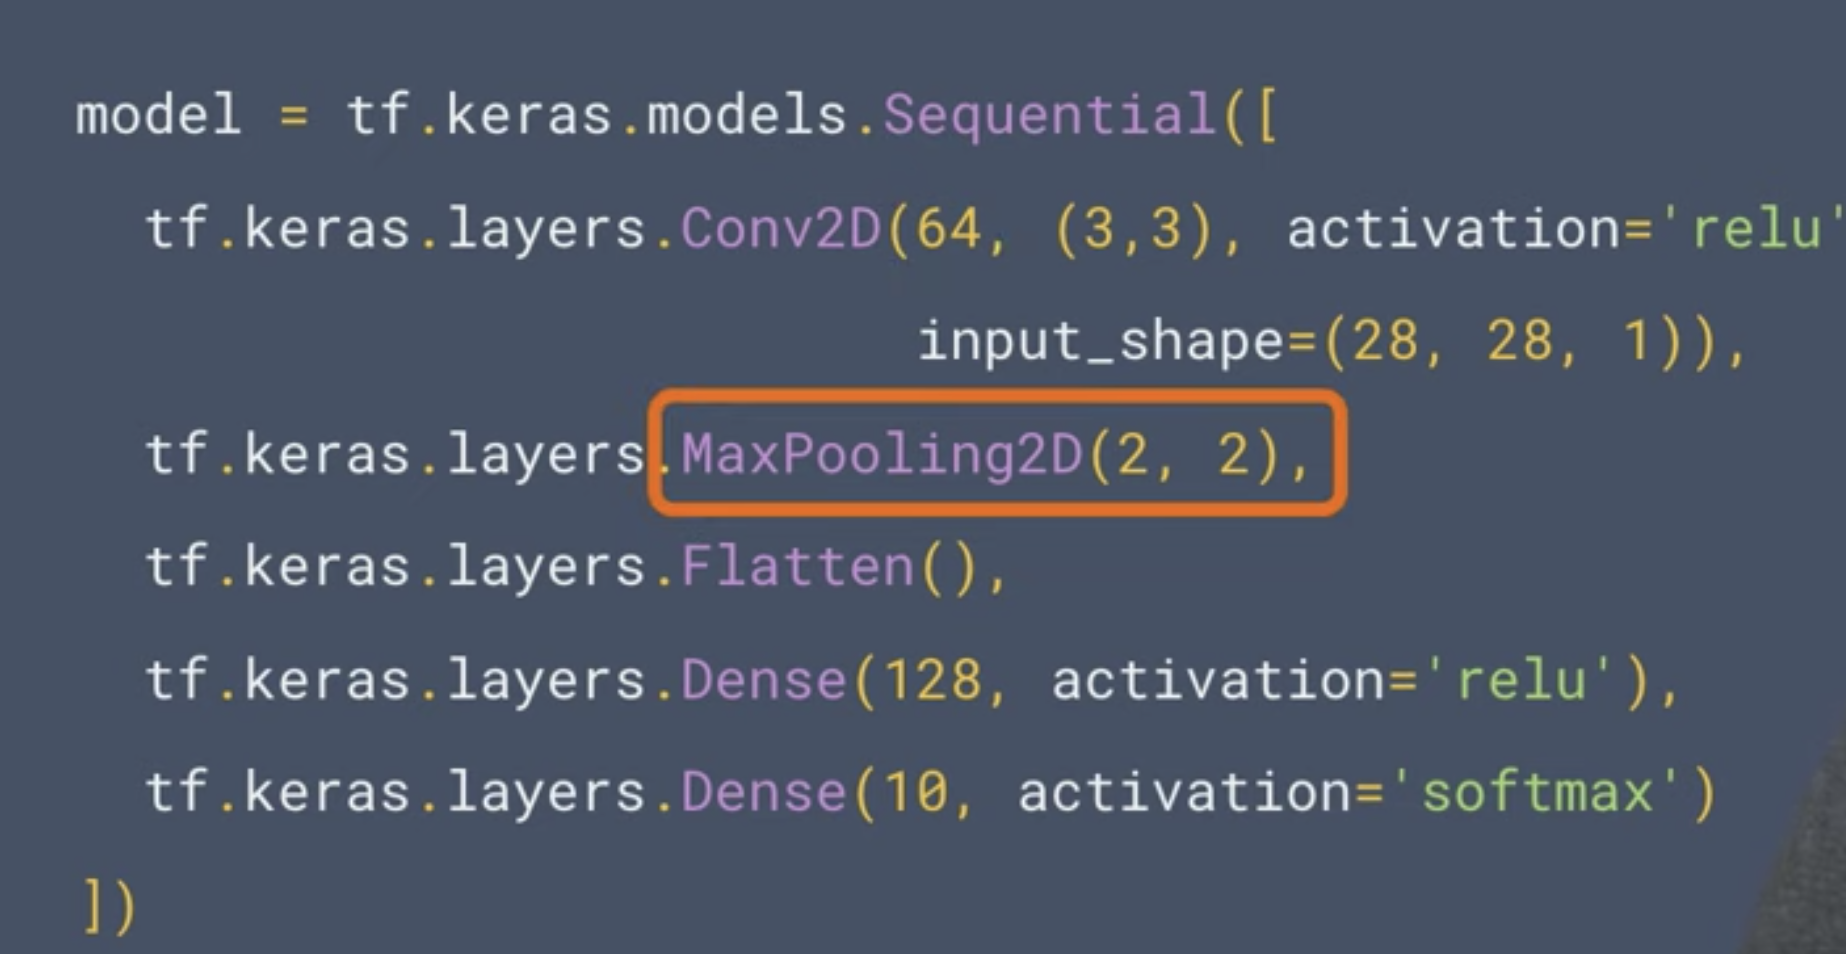
\includegraphics[width=0.4\linewidth]{img/code.png}
      \caption{Code}
      \label{fig:snn}
    \end{figure}
    \paragraph{}
    Now,lets take a look at the code to build a convolutional network like this. We have a flattened input that`s fed into a dense layer that intern is fed into the final dense layer that is our output. Notice we haven`t specified the input shape. That`s because i will put a concolutional layer on top of it like this. This layer takes the input so we specify the input shape, and we. are telling it to generate 64 filters with this parameter.
    \vspace{10mm}
    \begin{figure}[h!]
      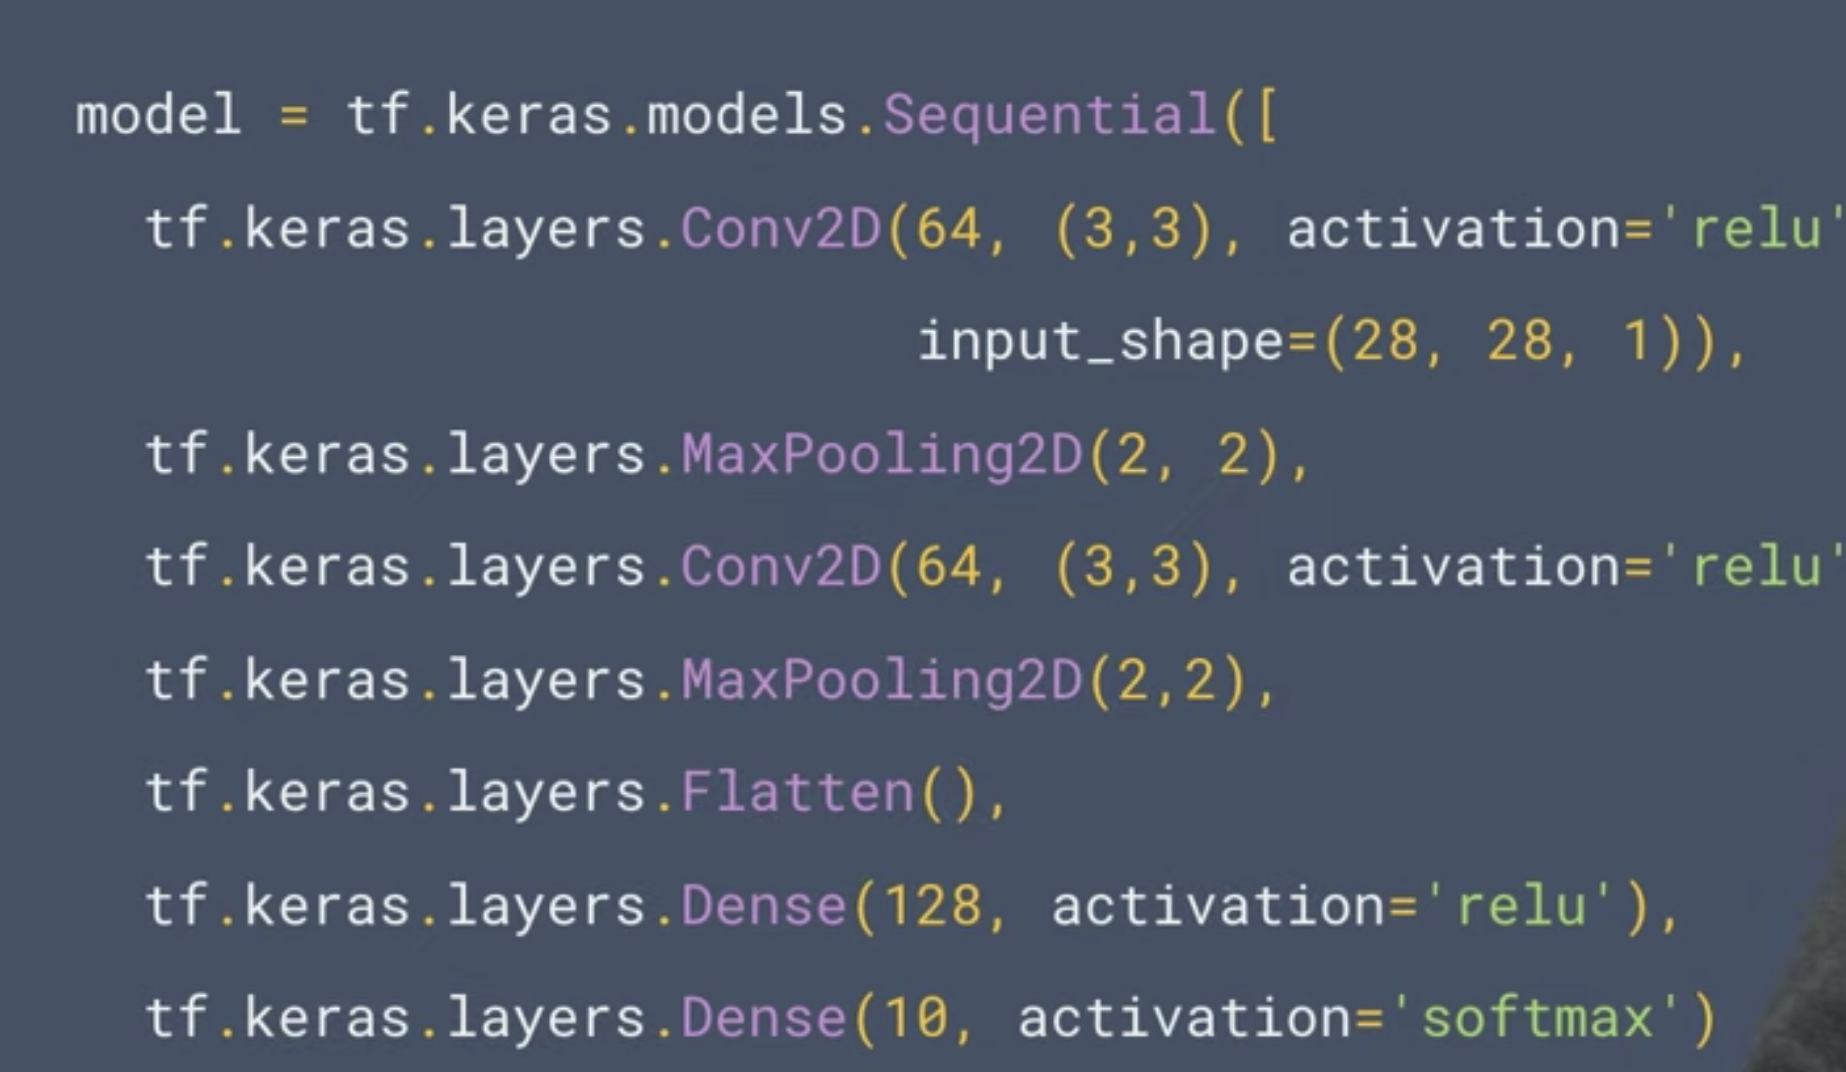
\includegraphics[width=0.4\linewidth]{img/code-stack.png}
      \caption{Code Stack}
      \label{fig:snn}
    \end{figure}
    \paragraph{}
    That is, it will generate 64 filters and multiply each of them across the image, than each epoch will figure out which filters gave the best signals to help match the images to their labels in much the same way it learned which parameters worked best in the dense layer. The max pooling to compress the image and enhance the features looks like this, and we can stack convolutional layer on top of each other to really break down the image and try to learn from very abstract features like this.
    \paragraph{}
    With this methodology your network starts to learn based on the features of the image instead of just the row patterns of pixels. Two sleeves, it`s a shirt. Two short sleeves, it`s a t-shirt. Sole and laces, it`s a shoe ets. Now we are still looking at just the simple images of fashion but the principles into more complex images. 



  \newpage
  \section{Recurrent Neural Network}
  Recurrent neural networks are learning model with a simple structure and a built-in feedback loop, allowing it to act as a forecasting engine. 
  Recurrent neural networks, or RNNs, have a long history, but their recent popularity is mostly due to the works of Juergen Schmidhuber,  Sepp Hochreiter, and Alex Graves. Their applications are extremely versatile, ranging from speech recognition to driverless cars.
  \subsection{How does it Work}
    \paragraph{}
    All the nets we’ve seen up to this point have been feedforward neural networks. In a feedforward neural network, signals flow in only one direction from input to output, one layer at a time. In a recurrent net, the output of a layer is added to the next input and fed back into the same layer, which is typically the only layer in the entire network. You can think of this process as a passage through time – shown here are 4 such time steps. At t = 1, the net takes the output of time t = 0 and sends it back into the net along with the next input. The net repeats this for t = 2, t = 3, and so on. Unlike feedforward nets, a recurrent net can receive a sequence of values as input, and it can also produce a sequence of values as output. The ability to operate with sequences opens up these nets to a wide variety of applications.

    \begin{figure}[h!]
      \begin{center}
        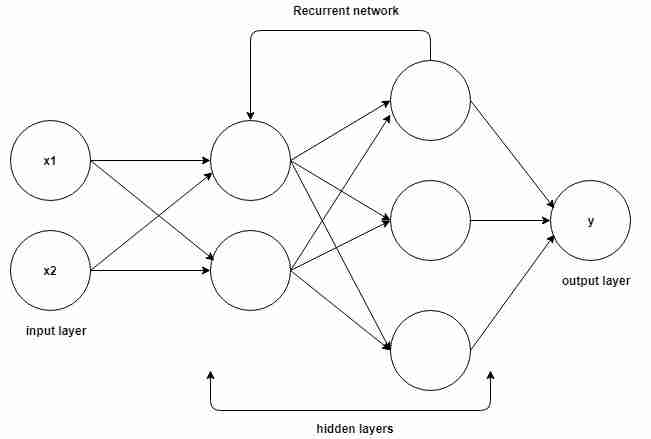
\includegraphics[width=0.8\linewidth]{img/Recurrent.jpeg}
        \caption{Recurrent Neural Network.}
        \label{fig:snn}
      \end{center}
    \end{figure}
    
    \paragraph{}
    Here are a few examples. When the input is singular and the output is a sequence, a potential application is image captioning. A sequence of inputs with a single output can be used for document classification. When both the input and output are sequences, these nets can classify videos frame by frame. If a time delay is introduced, the net can statistically forecast the demand in supply chain planning. Like we’ve seen with previous deep learning models, by stacking RNNs on top of each other, you can form a net capable of more complex output than a single RNN working alone.
    \subsubsection{Vanishing Gradient issue}
    Typically, an RNN is an extremely difficult net to train. Since these nets use backpropagation, we once again run into the problem of the vanishing gradient. Unfortunately, the vanishing gradient is exponentially worse for an RNN. The reason for this is that each time step is the equivalent of an entire layer in a feedforward network. So training an RNN for 100 time steps is like training a 100-layer feedforward net – this leads to exponentially small gradients and a decay of information through time.
    \begin{figure}[h!]
      \begin{center}
        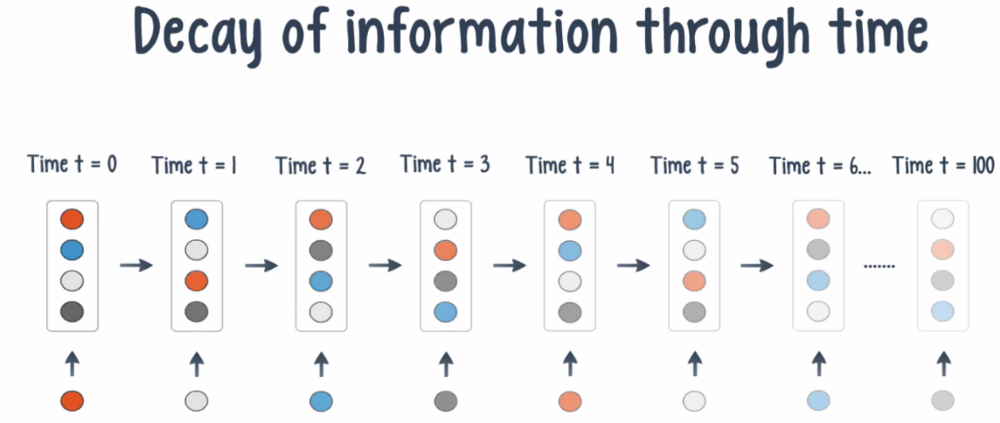
\includegraphics[width=0.8\linewidth]{img/vanishing-gradient.png}
        \caption{Vanishing Gradient.}
        \label{fig:snn}
      \end{center}
    \end{figure}
    
    \paragraph{}
    There are several ways to address this problem - the most popular of which is gating. Gating is a technique that helps the net decide when to forget the current input, and when to remember it for future time steps. The most popular gating types today are GRU and LSTM. Besides gating, there are also a few other techniques like gradient clipping, steeper gates, and better optimizers.

    \begin{figure}[h!]
      \begin{center}
        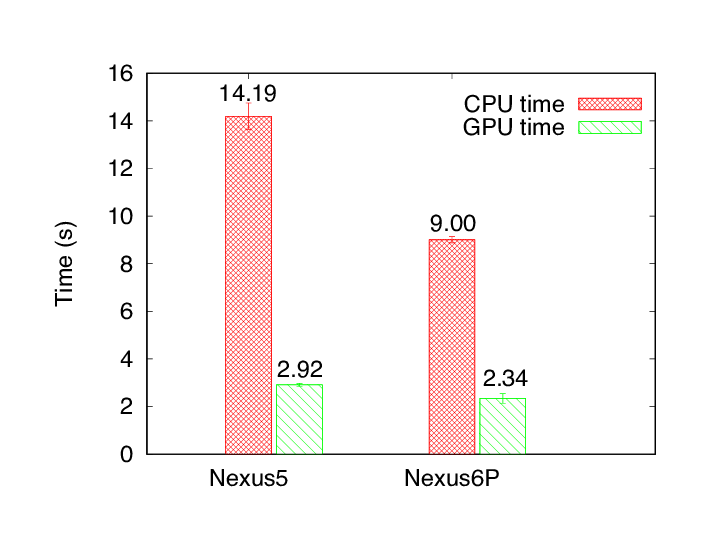
\includegraphics[width=0.8\linewidth]{img/rnn-gpu-cpu.png}
        \caption{LSTM GPU vs CPU.}
        \label{fig:snn}
      \end{center}
    \end{figure}
    \subsubsection{Gpu vs Cpu}
    When it comes to training a recurrent net, GPUs are an obvious choice over an ordinary CPU. This was validated by a research team at Indico, which uses these nets on text processing tasks like sentiment analysis and helpfulness extraction. The team found that GPUs were able to train the nets 250 times faster! That’s the difference between one day of training, and over eight months! So under what circumstances would you use a recurrent net over a feedforward net? We know that a feedforward net outputs one value, which in many cases was a class or a prediction. A recurrent net is suited for time series data, where an output can be the next value in a sequence, or the next several values. So the answer depends on whether the application calls for classification, regression, or forecasting.

  \newpage
  \section{Time series Data}
    \paragraph{}
    In order of increasing complexity we can think of time series data as a sequence of data points that measure the same thing over an ordered period of time. Another way of thinking about it, is that it's a series of numeric values, each with its own timestamp defined by a name and a set of label dimensions.
    \paragraph{} 
    We're seeing this type of data set become more common, in fact if we look at developer usage patterns in the past two years time series databases have emerged as the fastest growing category of databases.
    
    
    
    \paragraph{}
    Time series forecasting is performed in nearly every organization that works with quantifiable data. Retail stores forecast sales. Energy companies forecast reserves, production, demand, and prices. Educational institutions forecast enrollment. Goverments forecast tax receipts and spending. International financial organizations forecast inflation and economic activity. The list is long but the point is short - forecasting is a fundamental analytic process in every organization. The purpose of this example is to help with visualization of a Time Series Graph of an airline Company.
    \begin{figure}[h!]
      \begin{center}
        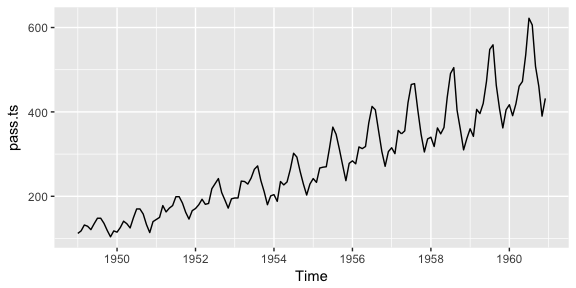
\includegraphics[width=0.8\linewidth]{img/unnamed-chunk-6-1.png}
        \caption{TimeSeries Data Example.}
        \label{fig:snn}
      \end{center}
    \end{figure}

    \paragraph{} 
    Well smart homes monitor data points like the temperature, number of people in the house and energy usage, Amazon monitors how its many assets are moving across the world with a fine-grained level of precision and efficiency that makes same-day delivery possible. All of these applications have one thing in common, they rely on a form of data that measures how things change over time. 
    \paragraph{}
    Usually time series data sets have three commonalities. The data that does arrive is recorded as a new entry, it arrives in time order and time is a primary axis. These data sets are generally append-only the data that has been reported doesn't change. Since it was recorded at some point in the past, time series data sets are different than just having a time field as a column in a data set. In that, when we collect a new data point for time series data we have to create a brand new row for it. Only by doing this will we be able to track all changes to a system over time. Recording data points over a series of time allows us to analyze how something has changed in the past monitor, how is changing in the presence and even predict how it could change in the future.
    \paragraph{} 
    Recurrent neural networks are able to learn how to make predictions in sequences of data and a variance of recurrent networks called long-short term memory networks are able to learn from even longer sequences of data. We can treat our data set as a supervised problem if we'd like and use an LS TM network to predict our target.

\vspace{30mm}
\section{Convolutional and Recurrent neural networks applied to sequential data}
When it comes to neural networks architectures, recurrent neural networks have traditionally been the go-to method for working with sequential data, such as text, speech, audio, video, etc. Usually convolutional neural networks are not even considered for these tasks. In recent years, however, there has been an increasing amount of research and practical applications utilizing convolutional neural networks for sequence analysis and prediction.
  \paragraph{}
  Bai, Kolter and Koltun (2018) [Bai, S., Kolter, J. Z., \& Koltun, V. (2018). An empirical evaluation of generic convolutional and recurrent networks for sequence modeling. arXiv preprint arXiv:1803.01271.] did extensive testing and comparison between state-of-the-art LSTM and GRU architectures, and a convolutional neural network in a wide variety of different classification tasks and datasets. They found out that the convolutional architecture substantially outperformed both recurrent architectures in all of the tasks. RNN:s are often regarded as well-suited for sequential data particularly because of their ability to retain temporal information. However, the convolutional neural network was able to retain information with 100 \% accuracy across all sequence lengths, while both of the recurrent networks quickly degenerated into random guessing.
  \begin{figure}[h!]
    \begin{center}
      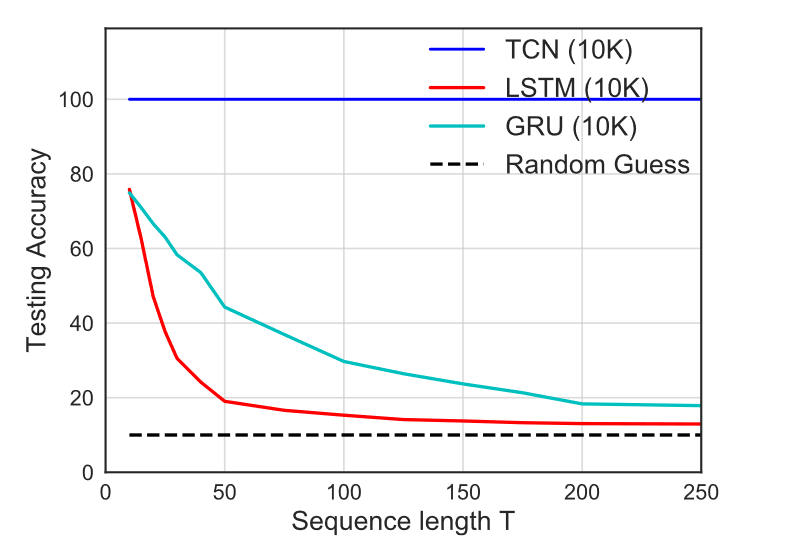
\includegraphics[width=0.8\linewidth]{img/image5.png}
      \caption{Accurrancy Graph.}
      \label{fig:snn}
    \end{center}
  \end{figure}
  \paragraph{}
  In a 2018 paper (Borovykh, A., Bohte, S., \& Oosterlee, C. W. (2018). Dilated convolutional neural networks for time series forecasting. Journal of Computational Finance, Forthcoming.) Convolutional neural network based on Google’s wavenet architecture was compared to LSTM in predicting financial data, which is noisy, chaotic, and very hard to make predictions from. The CNN architecture was more successful in finding underlying patterns from the data and was less susceptible to overfitting. Recurrent networks are also more complex and computationally demanding, which is a big downside in production environments.
  \newpage
  \section{Practical example}
  I our practical example we compared the performance of convolutional and recurrent neural networks, specifically the LSTM (long-short-term memory) variant of the recurrent neural network, which is supposed to address the issue of vanishing gradients present in regular RNN:s. We used a 1-dimensional convolutional neural network, which is more optimized for sequence and time series analysis, as opposed to the 2d CNN, which is more commonly used for image analysis and recognition related tasks. Both models were implemented in Python with the Keras library, using Tensorflow backend. Pandas, Numpy and Scikit Learn were also used in building the data pipeline. 
  \paragraph{}
  The data we used for the task was a weather dataset \href{https://www.kaggle.com/ktochylin/san-diego-every-minute-weather-indicators-201114}{(here)} collected from San Diego between 2011 and 2014 in one minute intervals, and it included indicators such as temperature, air pressure, humidity, wind speed, and others. In hindsight, this was probably not the best kind of dataset to use for benchmarking purposes, and the models we came up with certainly would not be useful for any kind of “real” analysis tasks. However, it was suitable for learning purposes. More useful results could probably have been obtained by combining this dataset with something else, like energy consumption.
  \paragraph{}
  We started by cleaning up the data by removing all of the NaN-values, setting datetime as index and discarding redundant and useless variables. To decide which variables to use, we first looked at the correlation matrix:

  \begin{figure}[h!]
    \begin{center}
      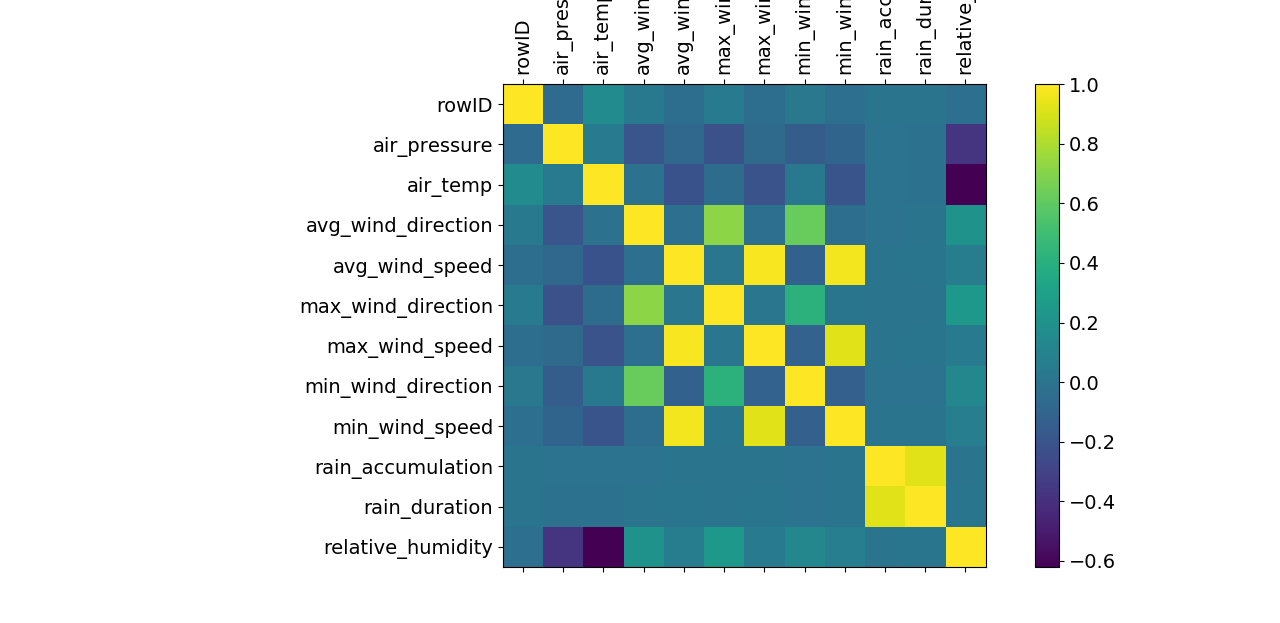
\includegraphics[width=\linewidth]{img/image3.png}
      \caption{Correlation Matrix.}
      \label{fig:snn}
    \end{center}
  \end{figure}
  You can immediately see that rain accumulation and duration, for example, are very closely correlated, which makes intuitive sense. Also, things like maximum wind speed and average wind direction seemed to be almost 1:1 correlated. After some consideration we settled on these variables:

  \begin{figure}[h!]
    \begin{center}
      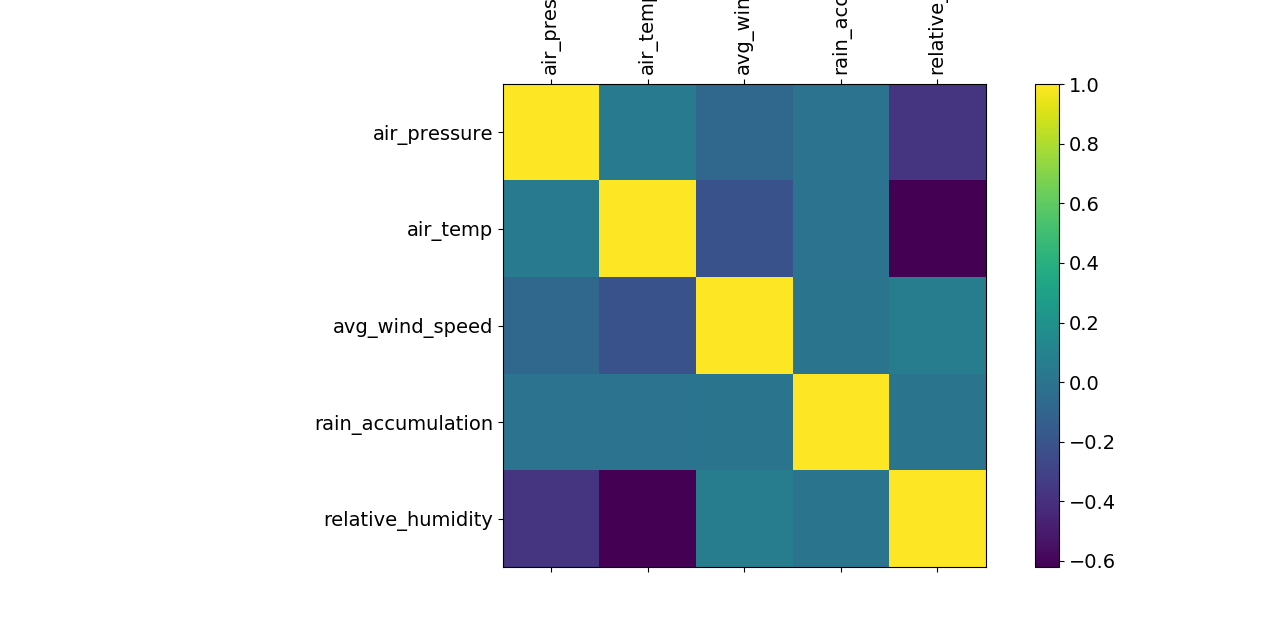
\includegraphics[width=\linewidth]{img/image2.png}
      \caption{Correlation Matrix with our variables.}
      \label{fig:snn}
    \end{center}
  \end{figure}
  Here is a graph of air temperature over the whole dataset:
  \begin{figure}[h!]
    \begin{center}
      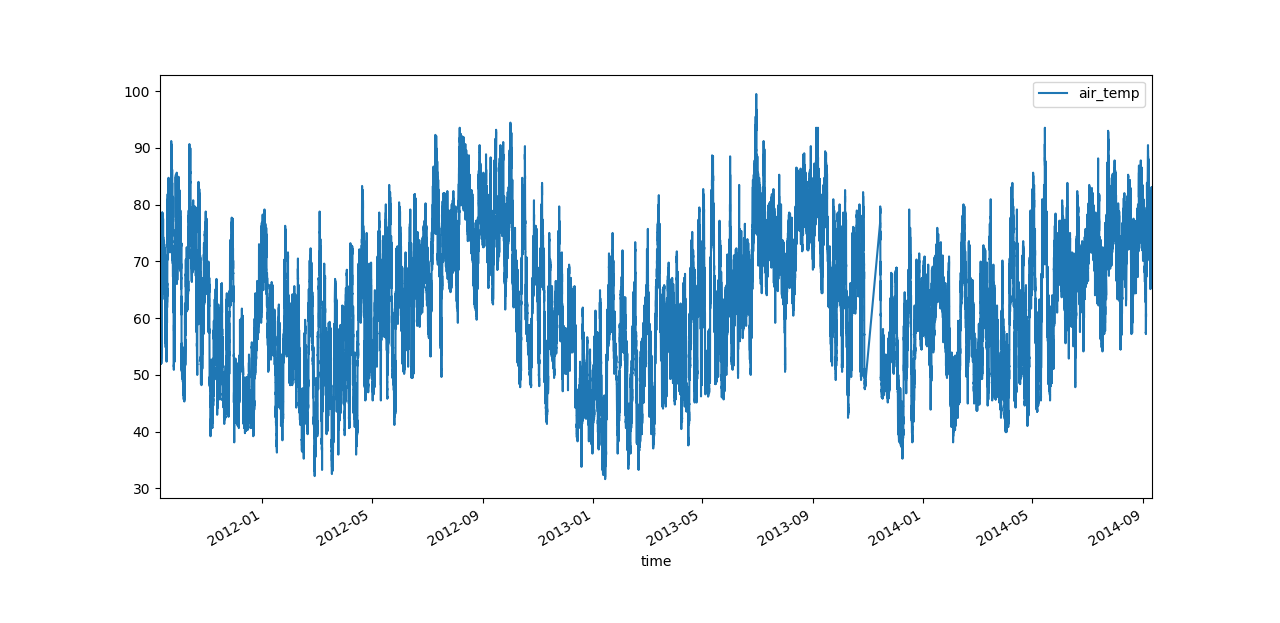
\includegraphics[width=\linewidth]{img/image6.png}
      \caption{Air Temperature Graph.}
      \label{fig:snn}
    \end{center}
  \end{figure}
  As for the prediction/classification task itself, we decided to try to predict if the average temperature for an arbitrarily long time interval in the future (60 minutes in our case) would go up or down, based on the weather activity from another arbitrarily long sequence (also 60 minutes in our case). In addition to the dataset itself probably not being optimal for the task, some other target variable and sequence lengths could probably have yielded better results. Our pipeline was built to be able to make sequences of any length, but we ended up not using any other values, because building of the sequences took too long with our hardware. The code could have probably been better optimized.
  \paragraph{}
  Before building the sequences, we split the whole dataset into training / validation / testing data, with a ratio of 60/20/20. Although we ended up only using the training and validation sets. After building the sequences we balanced the data, so for the training there would be equal number of instances from both classes. After that we normalized the data using sklearn.preprocessing.MinMaxScaler(). At the end of the pipeline we saved all datasets as numpy binary format for efficient storage to be used in our training pipelines.
  \paragraph{}
  The code for the balancing method in the data preprocessing pipeline was taken from \href{https://pythonprogramming.net/balancing-rnn-data-deep-learning-python-tensorflow-keras/}{here}
  \paragraph{}
  The code for the training itself was mostly trivial with both the CNN and RNN. We tried to make the architecture relatively simple, with 2 convolutional layers for the CNN and 2 LSTM layers for the RNN. Both had a flatten layer and 2 fully connected layers at the end. The loss function we used was binary crossentropy, because the task was binary classification, and the activation function used in the final layer was sigmoid, because it works with binary classification, as opposed to something like softmax, which is better for multi-class problems. We also added dropouts to each layer, which is a method used to reduce overfitting and improve model robustness by randomly dropping some amount of connections between neurons. Supposedly it’s not that widely used in research anymore.
  We ended up not doing much of hyperparameter optimization at all, at least not systematically, mostly because of time constraints. The comparison metrics used were accuracy and training time.
  \paragraph{}
  From the results we can see that the convolutional neural network performed much better, with both higher accuracy and lower loss. Training was also substantially lower. For some reason after few epochs, the LSTM got stuck at 50\% accuracy, even after adjusting several parameters. We suspect there might be a mistake in the code.
  \paragraph{}
  Training results for CNN:
  \begin{figure}[h!]
    \begin{center}
      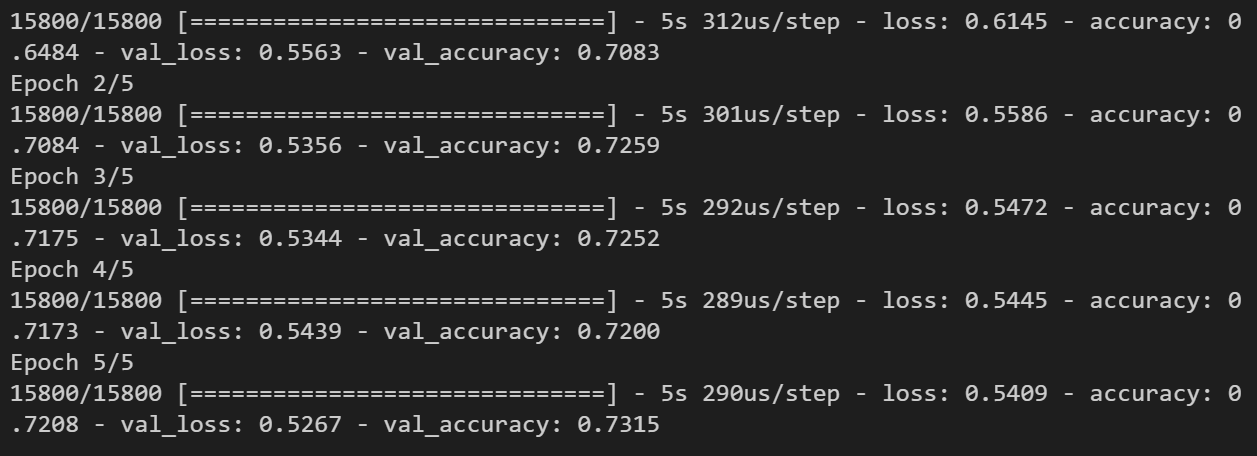
\includegraphics[width=\linewidth]{img/image4.png}
      \caption{CNN Results.}
      \label{fig:snn}
    \end{center}
  \end{figure}
  And LSTM:
  \begin{figure}[h!]
    \begin{center}
      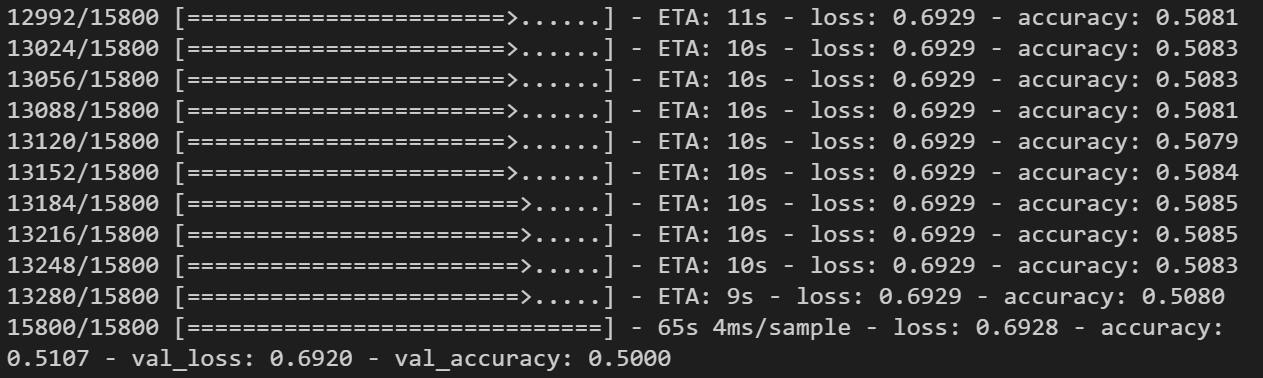
\includegraphics[width=\linewidth]{img/image1.png}
      \caption{LSTM Results.}
      \label{fig:snn}
    \end{center}
  \end{figure}

  \newpage
  \section{References}
  \href{http://www.cs.cmu.edu/~bhiksha/courses/deeplearning/Fall.2016/pdfs/Simard.pdf}{(1)Best practices for convolutional neural networks applied to visual document analysis, by:PY Simard, D Steinkraus, JC Platt - Icdar, 2003.}
  \newline
  \href{https://www.isca-speech.org/archive/interspeech_2010/i10_1045.html}{(2)Recurrent neural network based language model, by:T Mikolov, M Karafiát, L Burget, J Černocký, 2010}
  \newline
  \href{https://link.springer.com/chapter/10.1007/BFb0020283}{(3)Predicting time series with support vector machines, by: KR Müller, AJ Smola, G Rätsch, B Schölkopf, 1997}
  \newline
  \href{https://pythonprogramming.net/balancing-rnn-data-deep-learning-python-tensorflow-keras/}{(4)Balancing Recurrent Neural Network sequence data for our crypto predicting RNN - Deep Learning basics with Python, TensorFlow and Keras, by: SantDex}
  \newline
  \href{https://www.cv-foundation.org/openaccess/content_cvpr_2016/papers/Wang_CNN-RNN_A_Unified_CVPR_2016_paper.pdf}{(5)CNN-RNN: A Unified Framework for Multi-label Image Classification, by: Jiang Wang, Yi Yang, Junhua Mao, 2016}

  

\end{document}